\documentclass{article}

\usepackage{graphicx}
\usepackage{tikz}
\usepackage{tikzsymbols}
\usetikzlibrary{calc,patterns,shapes.geometric}
\pagestyle{empty}
\usepackage[margin=0pt]{geometry}
\geometry{papersize={14in,12in}}

\def\centerarc[#1](#2)(#3:#4:#5){\draw[#1] ($(#2)+({#5*cos(#3)},{#5*sin(#3)})$) arc (#3:#4:#5);}

\begin{document}
	\begin{figure}
		\centering
		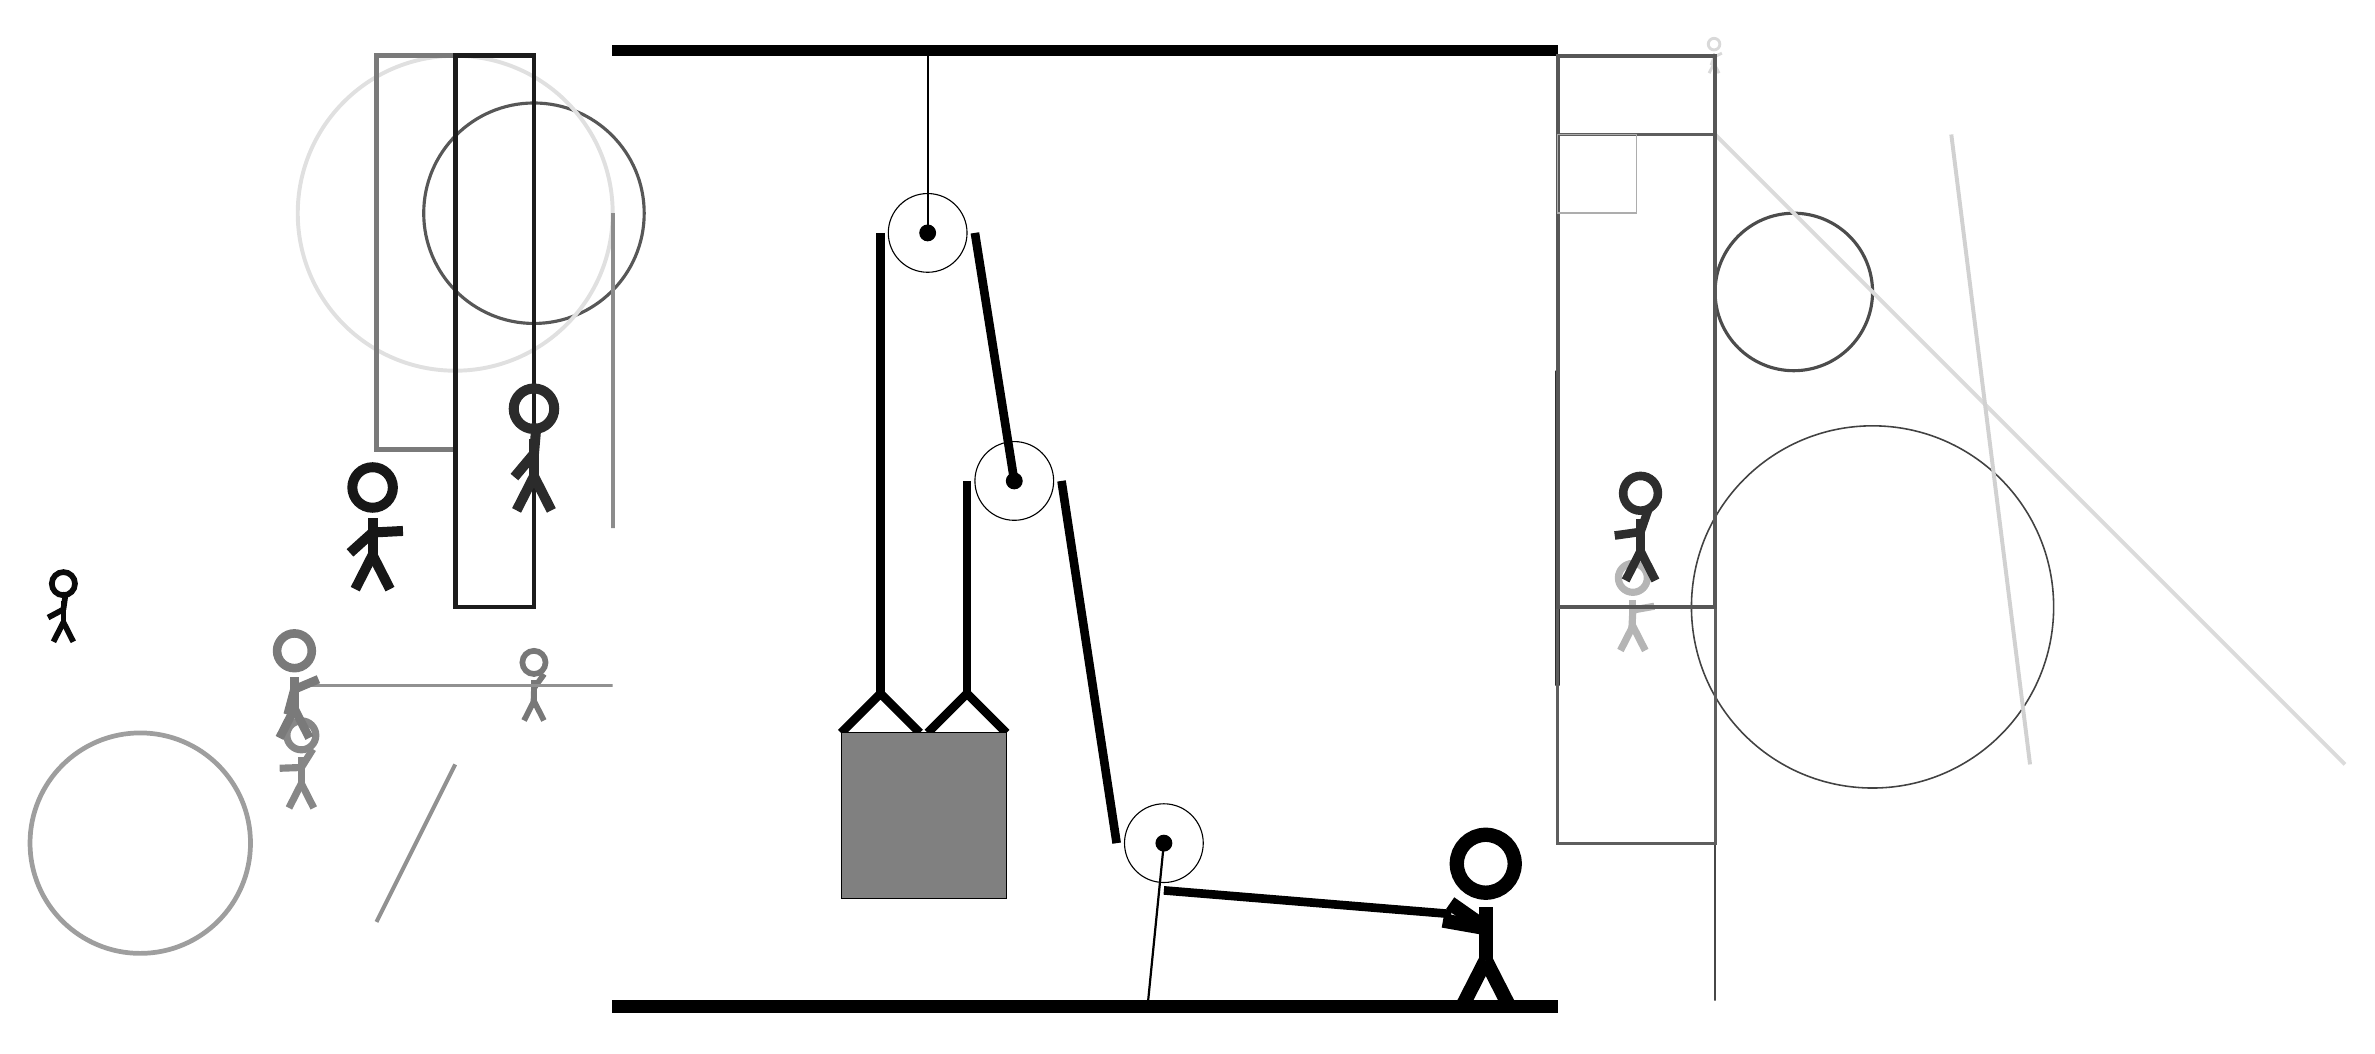
\begin{tikzpicture}
			%%%%% START %%%%%
			
			\draw[fill=black] (-2, 9) rectangle (10, 9.125);
			
			\draw (2, 6.75) circle (0.5);
			\draw[fill=black] (2, 6.75) circle (0.1);
			\draw[thick] (2, 6.75) -- (2, 9);
			
			\draw (3.1, 3.6) circle (0.5);
			\draw[fill=black] (3.1, 3.6) circle (0.1);
			
			\node[line width=0.4mm, color=black!53] at (-3, 1) {\Strichmaxerl[4][88][54]};
			
			\draw [line width=0.2mm, color=black!74](14, 2) circle (2.3);
			\draw [line width=0.4mm, color=black!66](-3, 7) circle (1.4);
			\node[line width=0.5mm, color=black!29] at (11, 2) {\Strichmaxerl[5][87][10]};
			\draw [line width=0.5mm, color=black!12](-4, 7) circle (2.0);
			\draw [line width=0.4mm, color=black!70](13, 6) circle (1.0);
			\draw[line width=0.6mm, color=black!52] (-4, 9) rectangle (-5, 4);
			\node[line width=0.3mm, color=black!96] at (-9, 2) {\Strichmaxerl[4][28][82]};
			\node[line width=0.4mm, color=black!82] at (11, 3) {\Strichmaxerl[6][8][71]};
			\draw[line width=0.4mm, color=black!43] (-2, 1) rectangle (-6, 1);
			\draw[line width=0.5mm, color=black!14](12, 8) -- (20, 0);
			\draw[line width=0.5mm, color=black!43](-5, -2) -- (-4, 0);
			\node[line width=0.5mm, color=black!91] at (-5, 3) {\Strichmaxerl[7][42][3]};
			\draw[line width=0.6mm, color=black!89] (-4, 9) rectangle (-3, 2);
			\node[line width=0.7mm, color=black!15] at (12, 9) {\Strichmaxerl[2][70][26]};
			\draw[line width=0.7mm, color=black!82] (10, 1) rectangle (10, 5);
			\draw[line width=0.5mm, color=black!45] (-2, 3) rectangle (-2, 7);
			\draw [line width=0.6mm, color=black!38](-8, -1) circle (1.4);
			\draw[line width=0.5mm, color=black!18](15, 8) -- (16, 0);
			\draw[line width=0.2mm, color=black!72] (12, -3) rectangle (12, 8);
			\node[line width=0.6mm, color=black!47] at (-6, 0) {\Strichmaxerl[5][2][58]};
			
			\node[line width=0.3mm, color=black!83] at (-3, 4) {\Strichmaxerl[7][50][85]};
			
			\node[line width=0.6mm, color=black!52] at (-6, 1) {\Strichmaxerl[6][75][23]};
			\draw[line width=0.4mm, color=black!63] (12, -1) rectangle (10, 8);
			\draw[line width=0.5mm, color=black!66] (12, 9) rectangle (10, 2);
			\draw[line width=0.2mm, color=black!32] (10, 8) rectangle (11, 7);
			
			
			\draw (5, -1) circle (0.5);
			\draw[fill=black] (5, -1) circle (0.1);
			\draw[thick] (5, -1) -- (4.8, -3);
			
			\draw[line width = 1.1mm]  (0.9, 0.4) -- (1.4, 0.9) -- (1.9, 0.4);
			\draw[line width = 1.1mm]  (2.0, 0.4) -- (2.5, 0.9) -- (3.0, 0.4);
			\draw[fill=black!50] (0.9, 0.4) rectangle (3.0, -1.7);
			
			\draw[line width = 1.1mm] (1.4, 6.75) -- (1.4, 0.9);
			\centerarc[line width = 1.1mm](2, 6.75)(0:180:0.6);
			\draw[line width = 1.1mm] (2.6, 6.75) -- (3.1, 3.6);
			\draw[line width = 1.1mm] (2.5, 3.6) -- (2.5, 0.9);
			\centerarc[line width = 1.1mm](3.1, 3.6)(0:180:0.6);
			\draw[line width = 1.1mm] (3.7, 3.6) -- (4.4, -1);
			\centerarc[line width = 1.1mm](5, -1)(180:270:0.6);
			\draw[line width = 1.1mm] (5, -1.6) -- (8.65, -1.9);
			
			\node at (9, -2) {\Strichmaxerl[10][-35][170]};
			
			\draw[fill=black] (-2, -3) rectangle (10, -3.15);
			
			%%%%% END %%%%%
		\end{tikzpicture}
	\end{figure}	
\end{document}